\documentclass[./../../paper.tex]{subfiles}
\graphicspath{{\subfix{./../../figures/}}}

\begin{document}
\citeauthor{hsieh_DiCE4ELInterpretingProcess_2021} has recently published a paper on the counterfactual generation of process data. They call their framework DiCE4EL and share many ideas with our framework. Therefore, we want to highlight the key differences and similarities. 

In their approach, they attempt to solve various issues that we have also highlighted in \autoref{sec:challenges}. Furthermore, they do so by incrementally generating the model in sequential order. However, unlike \citeauthor{oberst_CounterfactualOffPolicyEvaluation_2019}, whose solution creates counterfactuals for every step in the sequence, \citeauthor{hsieh_DiCE4ELInterpretingProcess_2021} focus on critical decision points they call milestones. 

To gain a better understanding, it is important to outline the event log the authors use briefly. It was taken from a Dutch bank which processes loan applications in which customers request a certain amount of money. The activities are related to either application states or manual work activities. The application states consist of tasks generated by a machine and manual work activities produced by humans. Hence, the manual work items occur in reference to the application state. For instance, if the loan application is in a \emph{pre accepted} state, then the next events are often produced by humans reviewing the state. Those events are essentially sub-events of the application state. Human activities do not have to happen sequentially. They can occur in parallel. The moment all manual work items conclude marks the decision for the next application state. For instance, from \emph{pre accepted} to \emph{accepted}. Now, to understand why the milestone approach works requires knowing that an application loan process will change to a rejection state, for instance, if all manual work items are completed. There will not be applications that suddenly switch to another state, although the work items of a previous state have not concluded yet. Thus, one can split the entire sequence into subsequences or ignore the sub-events, reducing the search space significantly. 

One issue with this approach is the fact that one would first have to identify these milestones. Hence, a crucial distinction to our proposed framework is their dependence on knowledge about the true process, as displayed in this section. Our framework does not leverage structural information about the true process model in question. We believe this is the core contribution in contrast to their approach.

\begin{figure}[htbp]
    \centering
    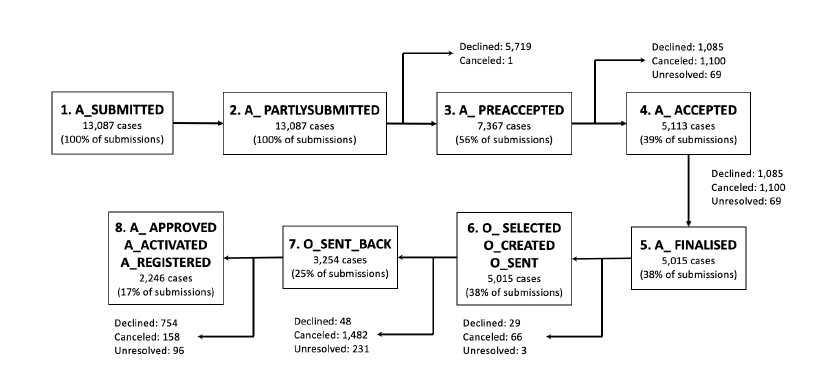
\includegraphics[width=\textwidth]{figures/milestones.png}
    \caption{Milestones of loan application process captured in BPIC2012 as
    identified in \cite{bautista_ProcessMiningDrivenOptimization_2012}}
    \label{fig:milestones}
\end{figure}

However, similarities between both frameworks do exist. Mainly, our approach also relies on the prediction scores of the model we attempt to explain. Similar to \citeauthor{hsieh_DiCE4ELInterpretingProcess_2021}, we incorporate these scores into our quality measure. 

% The next difference stems from how DiCE4EL operationalizes the quality criteria of their counterfactuals and on what bases they optimize their algorithm. \optional{we discuss those after discussing our operationalisation in \autoref{sec:viability}}




\end{document}